% -*- root: ../distributed_hosting_whitepaper.tex -*-

In this section the complete flow behaviour of the Framework for the basic
scenarios is presented. The analysis is based on the following scenarios:

\begin{enumerate}
\item In the first scenario, some user tries to access a webpage whose creator is up and running.
\item In the second scenario, the creator of the requested page is offline.
Nevertheless the node that makes the request has already the blockchain of that page.
\item In the third scenario the owner of the requested page is offline and besides, the node who
makes the request, does not host this web page.
\end{enumerate}

\subsection{Page request for a page who's owner is online}

\begin{figure}[htp]
\center
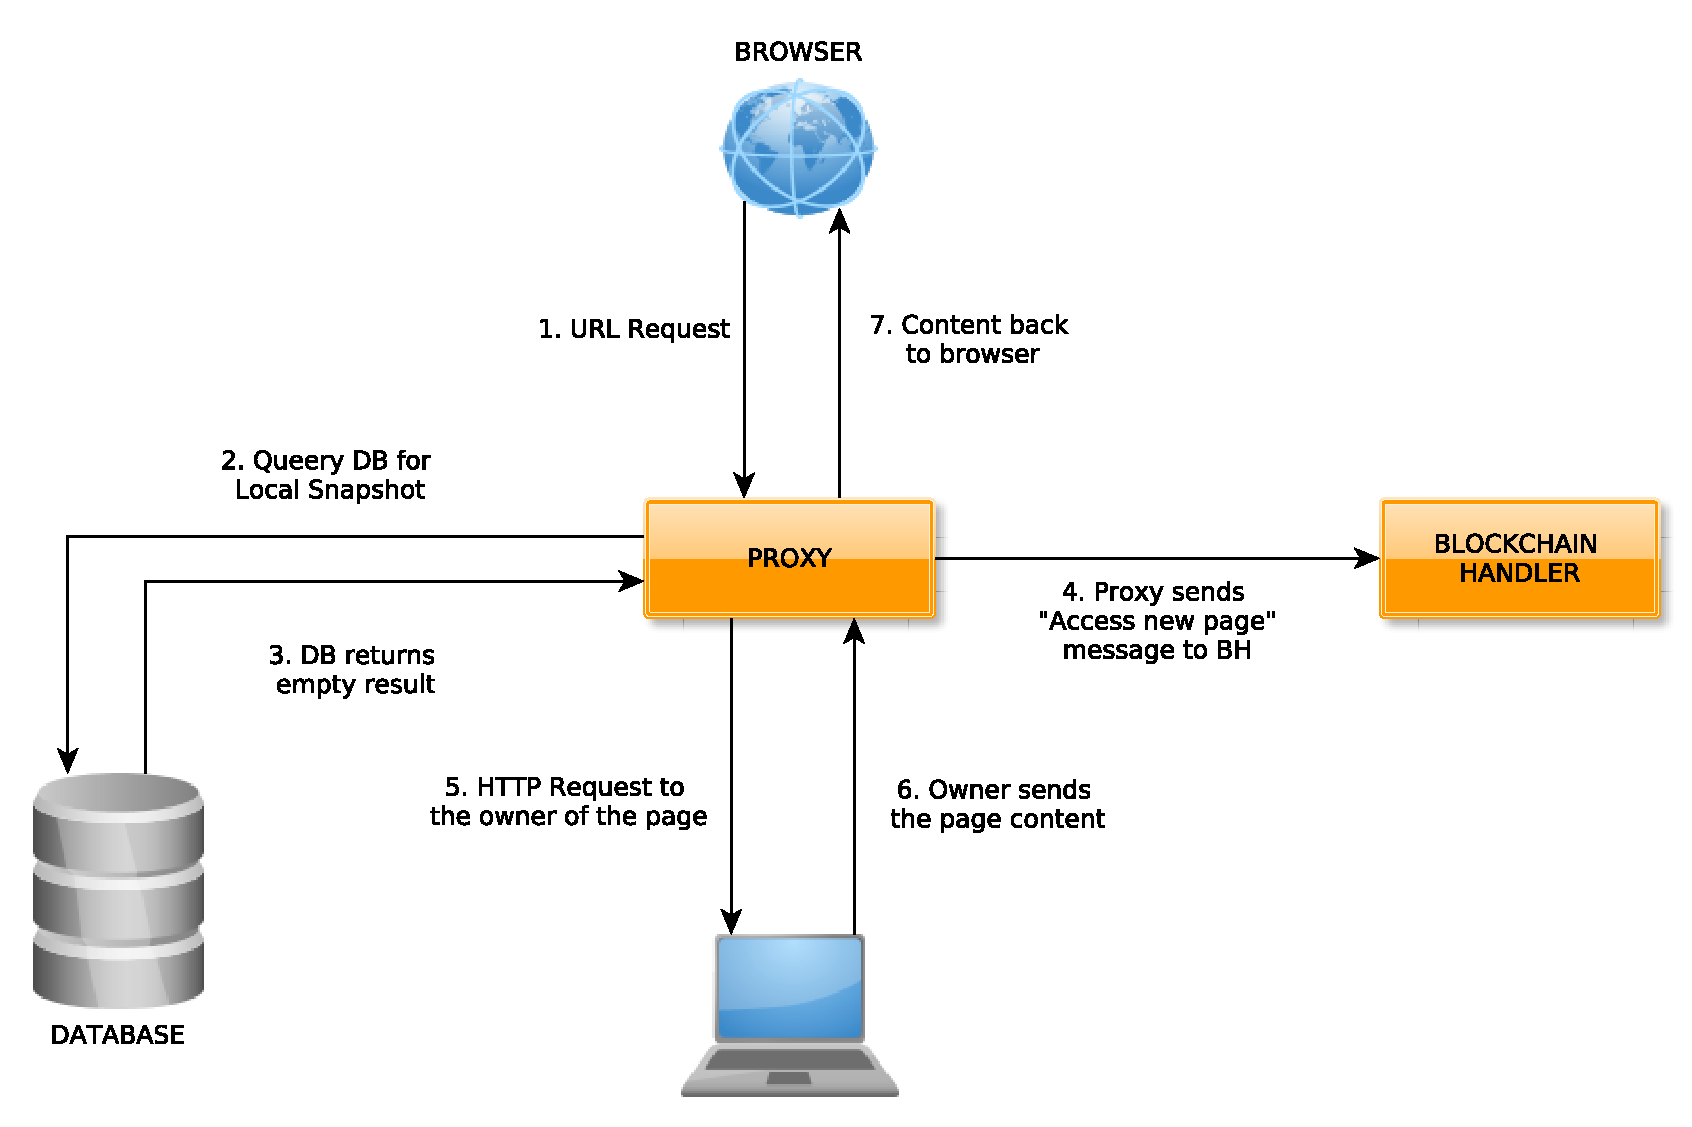
\includegraphics[width=0.5\textwidth]{pictures/fetch_page_online_creator.pdf}
\caption{First access of a web page whose creator is online.}
\label{fig:online_creator}
\end{figure}

In particular, when the user types the \texttt{url} of his choice in his browser the \texttt{Proxy} is
triggered and makes a query to the local database. The local database returns an empty result,
which is interpreted as absence of a stored snapshot and the blockchain for this page.
Accordingly, the proxy sends a message to the \texttt{Blockchain Handler} that is going to access
a web page for the first time and makes an \texttt{HTTP} request to the owner of the web page.
The message to the \texttt{Blockchain Handler} is essential because this is the component that stores
statistics and decides which pages are hosted. Finally, the owner responds to the \texttt{HTTP} request
and the user accesses the page.

\subsection{Page request for a page who's owner is offline}

\begin{figure}[htp]
\center
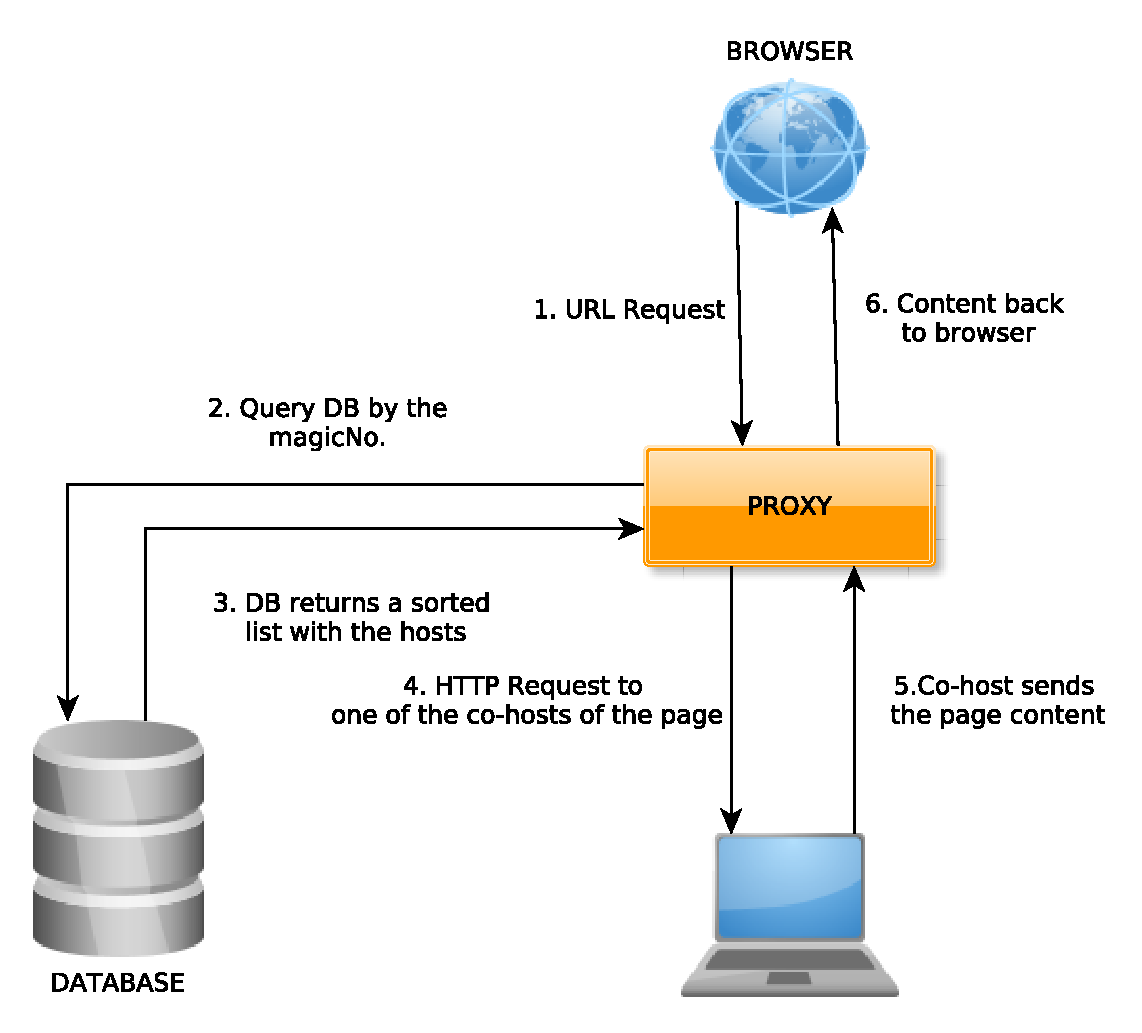
\includegraphics[width=0.4\textwidth]{pictures/fetch_page_offline_creator.pdf}
\caption{A node fetches a page from a co-host because its creator is offline.The
blockchain of the page is stored locally.}
\label{fig:offline_creator}
\end{figure}

In this case, when the \texttt{url} of the requested page is typed on the
browser, the \texttt{Proxy} is triggered. The database is then queried and
a sorted list of the known hosts of the target web page is returned. Typically,
the returned list is sorted by the criteria described in chapter
\textbf{to be specified/referenced.}

Accordingly, the \texttt{Proxy} makes \texttt{HTTP} requests to the hosts of
the list until it finds the first available host. This procedure should be
pretty quick because the higher a node is in the list the better the chances
are to be online and satisfy the request.


\subsection{First access to a web page who's owner is offline.}

\begin{figure}[htp]
\center
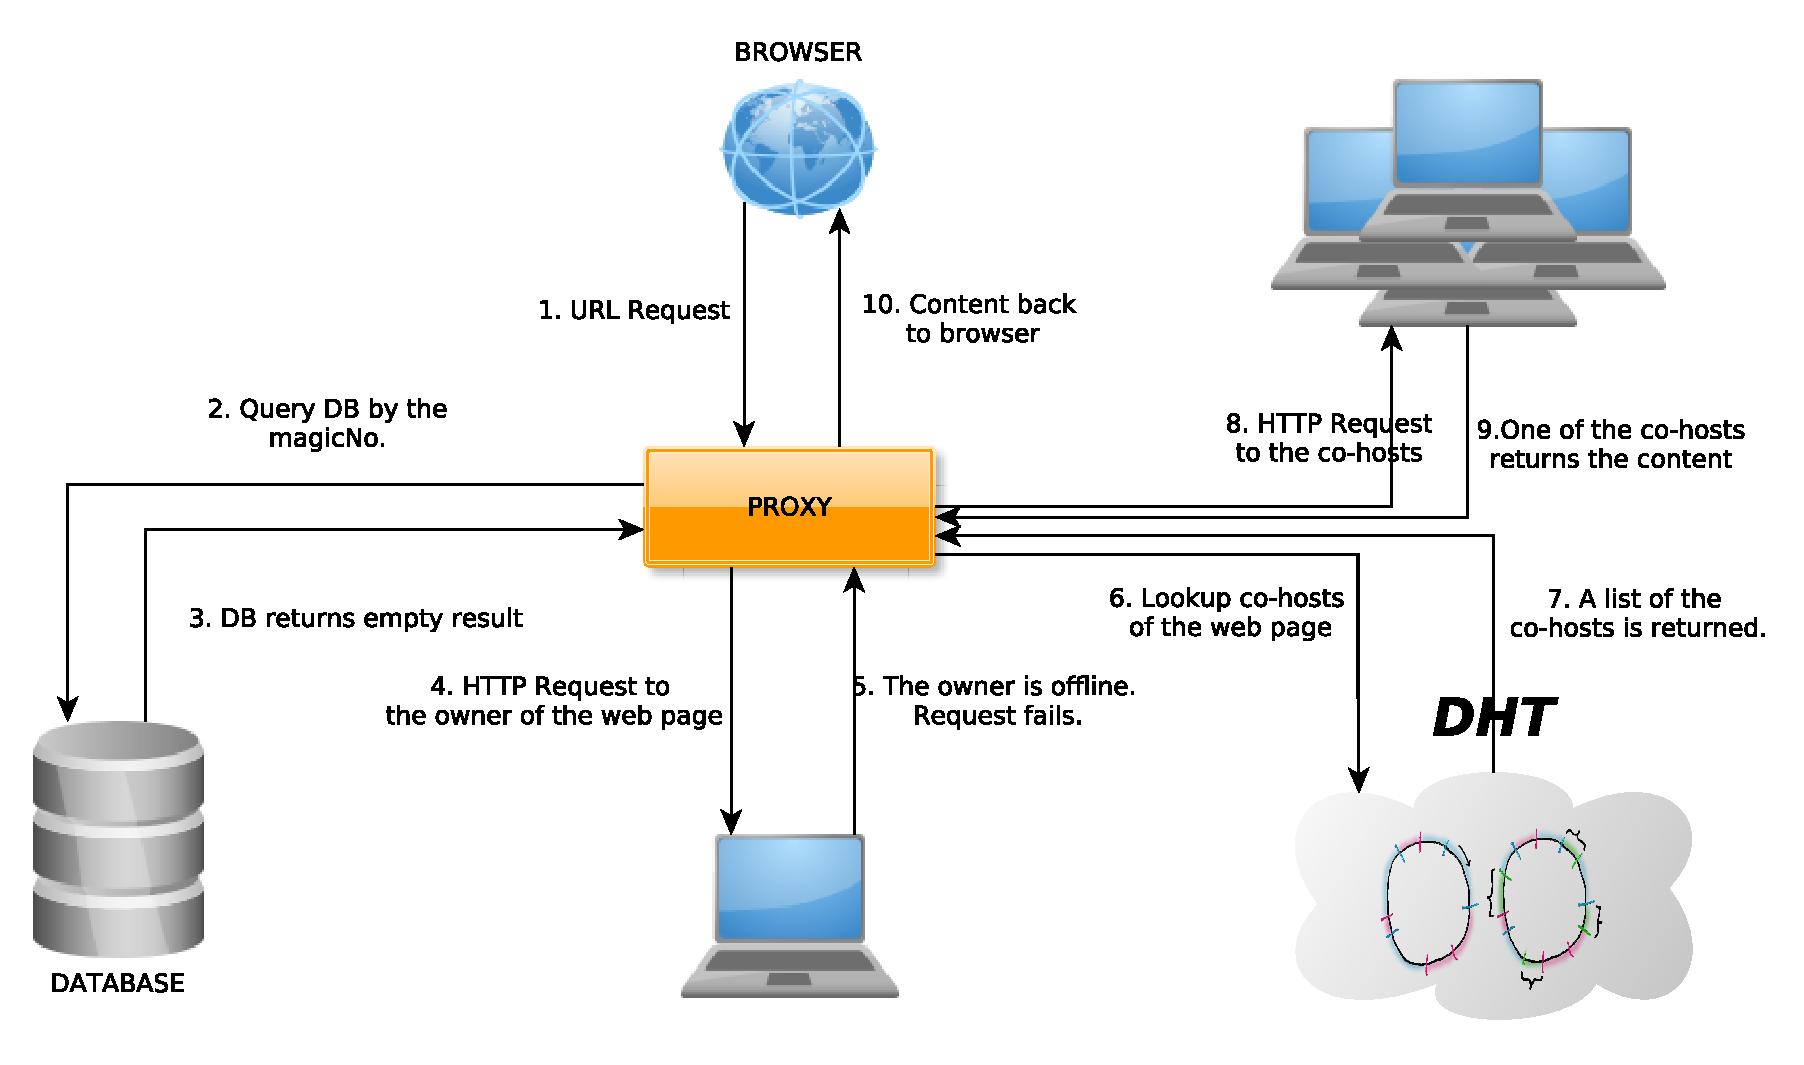
\includegraphics[width=0.6\textwidth]{pictures/fetch_page_offline_creator_no_blockchain_stored.pdf}
\caption{A node fetches a page from a co-host because its creator is offline.The list of
the co-hosts is provided by a DHT.}
\label{fig:offline_creator}
\end{figure}

In this scenario, the \texttt{Proxy} queries the local database for the requested \texttt{url}
and gets an empty result because the specific blockchain is not stored. Accordingly, the
\texttt{Proxy} sends an \texttt{HTTP} request to the owner of the web page which fails too
because the owner is offline.

Accordingly, the \texttt{Proxy} looks up the \texttt{Distributed Hash Table (DHT)} which is
the component that stores which nodes host which web page. The \texttt{DHT} returns a list
with the co-hosts of the web page and then the \texttt{Proxy} starts sending \texttt{HTTP}
requests to these nodes until it receives the content of the web page.
